%=======================================================================
% Supplementary Information for RG-SCSO (Iranian Journal of Computer
% Science submission). Font matches the main text: newtxtext/newtxmath
% (Times-like, pdflatex-compatible), not fontspec/unicode-math -- the main
% .tex now targets sn-jnl[pdflatex], so both files compile with the same
% standard pdfTeX engine.
%=======================================================================
\documentclass[9pt]{article}
\usepackage[a4paper,margin=25mm]{geometry}
\usepackage{newtxtext,newtxmath}
\usepackage{amsmath,graphicx,booktabs,multirow,rotating,hyperref}
\usepackage{placeins}
\graphicspath{{figures/}{./}}
\renewcommand{\thetable}{S\arabic{table}}
\renewcommand{\thefigure}{S\arabic{figure}}
\renewcommand{\thesection}{S\arabic{section}}
\title{Supplementary Information for: Relevance-Guided Binarization for
Parsimonious Feature Selection with Sand Cat Swarm Optimization}
\author{Bui Quang Huy, Duong Minh Son}
\date{}
\begin{document}
\maketitle

\FloatBarrier
\section{Proofs of Lemma 1 and Proposition 2}
\textbf{Proof of Lemma 1 (Leverage bound).} By the mean value theorem
there is a point $\xi$ strictly between $x_j$ and $x_j+\delta_j$ for which
$\Delta_j=T'(\xi)\,\delta_j$, so
$|\Delta_j|=|T'(\xi)|\,|\delta_j|\le\|T'\|_\infty\,|\delta_j|$; because
$|\tanh|$ fails to be differentiable only at the origin, applying the
theorem separately on each side of zero extends the bound to every
interval. Differentiating the two standard transfers gives
$\sigma'(x)=\sigma(x)(1-\sigma(x))=\tfrac{e^{-|x|}}{(1+e^{-|x|})^2}$ and
$|\tanh|'(x)=\operatorname{sech}^2(x)=\tfrac{4e^{-2|x|}}{(1+e^{-2|x|})^2}$,
whose maxima are $\tfrac14$ at $\sigma=\tfrac12$ and $1$ as $x\to0$, and
each decays away from the origin ($\sigma'(x)\le e^{-|x|}$,
$\big||\tanh|'(x)\big|\le 4\,e^{-2|x|}$). Substituting
$\|T'\|_\infty\le\varepsilon$ on a flat interval establishes the claim.

\textbf{Proof of Proposition 2 (Transition probability under the base
V-shaped transfer).} The identity $P_{\text{base}}\big(b_j^{(t+1)}\ne
b_j^{(t)}\mid
x_j^{(t)}\big)=T(x_j^{(t)})$ follows directly from the definition of the
\emph{base, unmodulated} V-shaped flip rule (a bit is flipped, independently
at each iteration, with probability equal to the transfer value); no further
argument is required because transition and flip are the same event under
this base rule. RG-SCSO's own rule replaces this base probability with the
relevance-modulated $p_j$ of Eq.~(2) of the main text, so this identity does
not apply to RG-SCSO directly (see Remark, main text). The
one-step bound $\big|\Delta P\big(b_j^{(t+1)}\ne b_j^{(t)}\big)\big|\le
\|T'\|_\infty\,|\delta_j|$ is then Lemma~1 restated in this coincidence.
Summing the per-step bound over $t=1,\dots,N$ and applying the triangle
inequality gives the cumulative bound
$\big|\sum_{t=1}^{N}\Delta P\big(b_j^{(t+1)}\ne b_j^{(t)}\big)\big|\le
\varepsilon\sum_{t=1}^{N}|\delta_j^{(t)}|$; expectation is linear, so the
bound on the sum of per-step probability differences is also a bound on
the difference in expected flip counts accumulated over the $N$ steps.

\textbf{What this does and does not establish.} Proposition 2 answers the
specific gap raised in review: because transition and flip coincide under
the rule used here, the local sensitivity bound of Lemma~1 is already a
bound on transition probability, and that bound composes linearly over
repeated sampling of the same bit, so the accumulated leverage of a
continuous-space perturbation over an entire saturated-regime run stays
controlled by $\varepsilon$ and does not grow without bound as $N$
increases. It does not establish that continuous-space enhancements are
ineffective: a perturbation applied while $T'$ is not small, or a
sufficiently large $\sum_t|\delta_j^{(t)}|$, can still accumulate a
non-negligible transition-probability shift. The result is a genuine,
expectation-level link from coordinate perturbation to discrete transition
dynamics, not a proof that washout is unavoidable.

\textbf{Scope of this result.} Lemma~1 establishes a local sensitivity
bound on how far a continuous-space perturbation can move a single flip
probability. Proposition~2 extends this to a cumulative bound over
repeated sampling of the same bit, showing the accumulated leverage stays
controlled by $\varepsilon$ in the flat, saturated regime rather than
growing without bound. Neither result proves that continuous-space
enhancements become uniformly ineffective once repeated stochastic
binarization is applied outside that regime, or that a probability change
of any size never accumulates into a discrete decision loss. We use
washout, throughout this paper, as a diagnostic framing motivated by these
bounds and corroborated empirically (main text Results; this document), not
as a formal guarantee that continuous-space enhancements must fail under
binary search.

\FloatBarrier
\section{Dataset characteristics}
\begin{table}[t]
\centering
\caption{Dataset characteristics (samples, features, classes).}
\label{tab:datasets}
\footnotesize
\begin{tabular}{lccc}
\toprule
Dataset & Samples & Features & Classes \\
\midrule
BreastEW & 683 & 9 & 2 \\
ColonCancer & 62 & 2000 & 2 \\
Diabetes & 768 & 8 & 2 \\
GermanCredit & 1000 & 20 & 2 \\
HeartDisease & 297 & 13 & 2 \\
IonosphereEW & 351 & 34 & 2 \\
KrVsKpEW & 3196 & 35 & 2 \\
Leukemia & 72 & 3571 & 2 \\
Lymphography & 148 & 18 & 4 \\
M-of-n & 1000 & 13 & 2 \\
Parkinsons & 195 & 22 & 2 \\
Sonar & 208 & 60 & 2 \\
SpectEW & 267 & 22 & 2 \\
TicTacToe & 958 & 9 & 2 \\
Vote & 232 & 16 & 2 \\
WDBC & 569 & 30 & 2 \\
WaveformEW & 5000 & 40 & 3 \\
Zoo & 101 & 16 & 7 \\
\bottomrule
\end{tabular}
\end{table}


\FloatBarrier
\section{In-sample accuracy and parsimony (optimistic upper bound)}
\label{sec:insample}
The main text reports held-out (leak-free) accuracy as the primary estimate.
For completeness, this section reports the
standard in-sample protocol, in which the relevance prior, search, and
reported metric share the same cross-validation folds; effect sizes here are
inflated relative to the held-out estimate (see main text Discussion).

\FloatBarrier
\section{Convergence behaviour}
\begin{figure}[htbp]
\centering
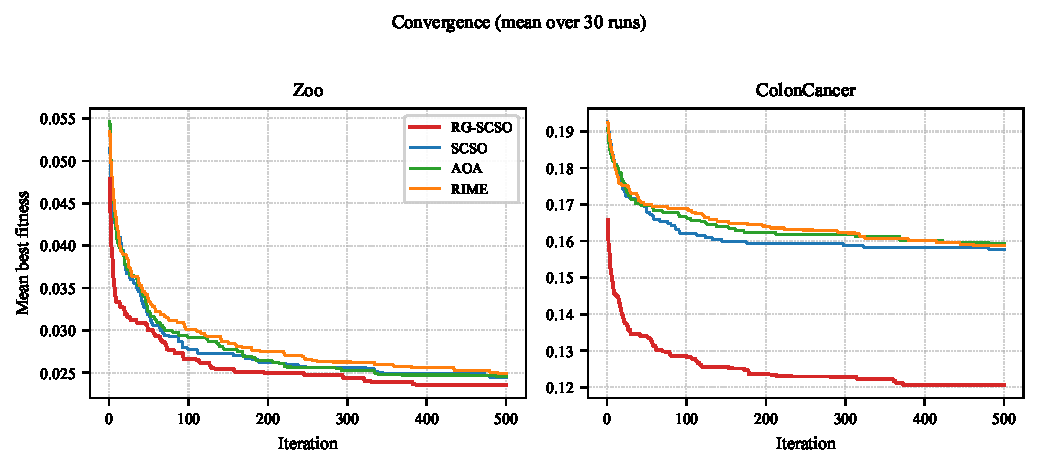
\includegraphics[width=0.92\textwidth]{convergence.pdf}
\caption{Mean best fitness versus iteration on a low-dimensional (Zoo) and a
high-dimensional (ColonCancer) dataset, averaged over 30 runs.}
\label{fig:conv}
\end{figure}

\FloatBarrier
\section{Exploration-safety diagnostic}
\begin{table}[t]
\centering
\caption{End-of-run population diversity and frozen-bit fraction, mean over 3 runs, for three relevance-bias settings: no relevance ($\gamma=0$, plain V-shaped), the default used throughout the paper ($\gamma=0.5$), and a maximal-bias stress test ($\gamma=1$). Diversity is the mean expected normalized Hamming spread $2\bar p(1-\bar p)$ across features; frozen fraction is the share of features on which every individual in the population agrees.}
\label{tab:diversity}
\footnotesize
\begin{tabular}{lcccccc}
\toprule
& \multicolumn{3}{c}{Diversity} & \multicolumn{3}{c}{Frozen fraction} \\
Dataset & $\gamma$=0 & $\gamma$=0.5 & $\gamma$=1 & $\gamma$=0 & $\gamma$=0.5 & $\gamma$=1 \\
\midrule
ColonCancer & 0.483 & 0.389 & 0.103 & 0.000 & 0.000 & 0.511 \\
WDBC & 0.482 & 0.437 & 0.303 & 0.000 & 0.000 & 0.111 \\
Zoo & 0.483 & 0.442 & 0.320 & 0.000 & 0.000 & 0.125 \\
\bottomrule
\end{tabular}
\end{table}

\begin{figure}[htbp]
\centering
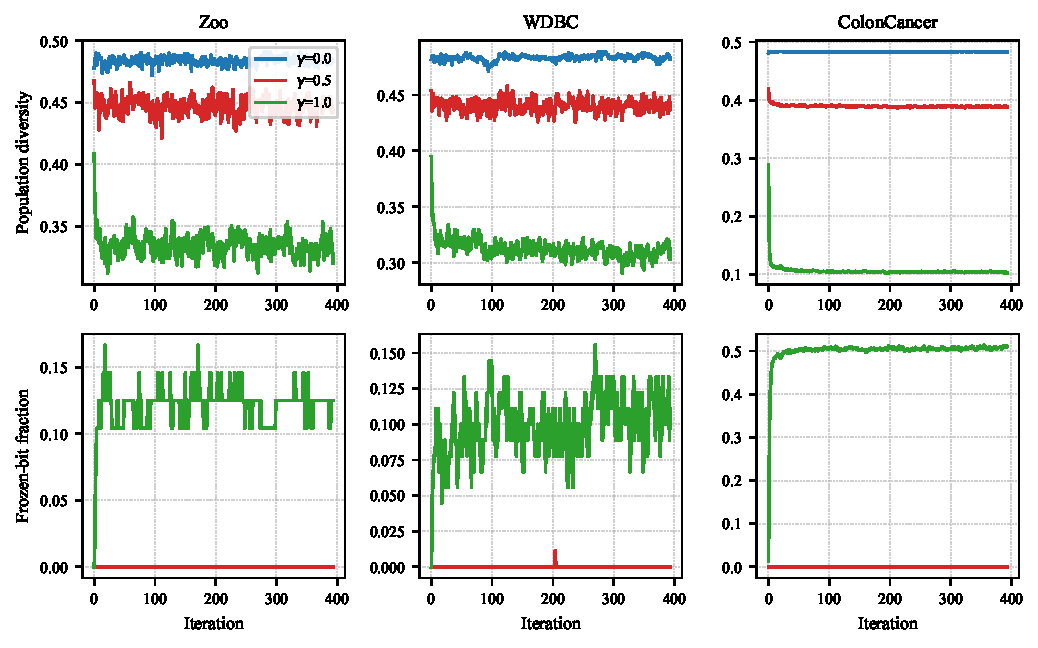
\includegraphics[width=0.92\textwidth]{diversity.pdf}
\caption{Population diversity and frozen-bit fraction versus iteration, for
$\gamma=0$, the deployed $\gamma=0.5$, and the stress-test $\gamma=1$, on
three datasets of increasing dimensionality.}
\label{fig:diversity}
\end{figure}

\FloatBarrier
\section{Preliminary washout study}
\begin{table}[t]
\centering
\caption{Preliminary washout study: mean accuracy of the continuous-enhanced SCSO (ECL-SCSO) vs.\ base SCSO over 30 runs; significance by Wilcoxon signed-rank at $\alpha=0.05$ (0 wins, 1 loss, 17 ties).}
\label{tab:washout}
\footnotesize
\begin{tabular}{lccc}
\toprule
Dataset & ECL-SCSO & SCSO & Sig.\ (Wilcoxon) \\
\midrule
BreastEW & 0.9484 & 0.9582 & n.s. \\
ColonCancer & 0.7727 & 0.7810 & n.s. \\
Diabetes & 0.7098 & 0.6937 & n.s. \\
GermanCredit & 0.7094 & 0.7099 & n.s. \\
HeartDisease & 0.7678 & 0.7759 & n.s. \\
IonosphereEW & 0.8464 & 0.8511 & n.s. \\
KrVsKpEW & 0.8019 & 0.8297 & n.s. \\
Leukemia & 0.9661 & 0.9619 & n.s. \\
Lymphography & 0.7689 & 0.7601 & n.s. \\
M-of-n & 0.7619 & 0.7698 & n.s. \\
Parkinsons & 0.8824 & 0.8985 & n.s. \\
Sonar & 0.8120 & 0.8122 & n.s. \\
SpectEW & 0.7876 & 0.7997 & n.s. \\
TicTacToe & 0.7164 & 0.6683 & n.s. \\
Vote & 0.8869 & 0.8930 & n.s. \\
WDBC & 0.9550 & 0.9619 & loss (p=0.017) \\
WaveformEW & 0.7407 & 0.7178 & n.s. \\
Zoo & 0.8763 & 0.8643 & n.s. \\
\bottomrule
\end{tabular}
\end{table}


\FloatBarrier
\section{Hyperparameter sensitivity}
\begin{table}[t]
\centering
\caption{Hyperparameter sensitivity (one-factor-at-a-time): mean accuracy and mean number of selected features over three datasets $\times$ 10 runs at a fixed NFE budget. $\gamma$ and $K$ are swept on the final (ORL-off) method; $\lambda$ and $w_o$ on the ORL-on variant (inert in the shipped method).}
\label{tab:sensitivity}
\footnotesize
\begin{tabular}{llcc}
\toprule
Parameter & Value & Mean Acc. & Mean \#Feat. \\
\midrule
$\gamma$ (RMS) & 0.00 & 0.9051 & 340.3 \\
 & 0.25 & 0.9117 & 262.8 \\
 & 0.50 & 0.9195 & 196.2 \\
 & 0.75 & 0.9285 & 119.5 \\
 & 1.00 & 0.9274 & 47.8 \\
\addlinespace
$K$ (UMR) & 2 & 0.9186 & 193.6 \\
 & 4 & 0.9192 & 195.5 \\
 & 8 & 0.9195 & 196.2 \\
 & 12 & 0.9195 & 196.3 \\
 & 16 & 0.9178 & 194.7 \\
\addlinespace
$\lambda$ (ORL) & 0.70 & 0.9225 & 193.3 \\
 & 0.90 & 0.9207 & 194.4 \\
 & 0.99 & 0.9223 & 193.4 \\
\addlinespace
$w_o$ (ORL) & 0.1 & 0.9198 & 190.3 \\
 & 0.3 & 0.9207 & 194.4 \\
 & 0.7 & 0.9225 & 195.9 \\
\bottomrule
\end{tabular}
\end{table}


\FloatBarrier
\section{Isolating the relevance contribution from adaptive transfers}
The table below reports binary particle-swarm and grey-wolf optimizers
equipped with published adaptive V-shaped transfers, run under the identical
protocol and budget as the main study but with no per-feature relevance
signal.

\begin{table}[t]
\centering
\caption{Confound-isolation against adaptive-transfer binary optimizers (bPSO/bGWO with the time-varying $|\tanh|$ transfer of Islam et~al.~\cite{islam2017tvtf} and the V4 transfer of Teng et~al.~\cite{teng2017avbpso}), same 18 datasets $\times$ 30 runs and budget as the main study. RG-SCSO does not lead on accuracy, yet selects the fewest features consistently. Best per column in bold; rank is over mean fitness.}
\label{tab:adaptive}
\footnotesize
\begin{tabular}{lcccc}
\toprule
Method & Mean Acc. & Mean \#Feat. & Mean Fitness & Rank \\
\midrule
\textbf{RG-SCSO (ours)} & 0.9009 & \textbf{91.3} & 0.1022 & 3.44 \\
bPSO-TVT & 0.9077 & 123.3 & 0.0961 & 2.78 \\
bGWO-TVT & 0.8998 & 157.2 & 0.1042 & 3.69 \\
bPSO-V4 & \textbf{0.9116} & 124.2 & \textbf{0.0921} & \textbf{1.39} \\
bGWO-V4 & 0.9001 & 159.0 & 0.1039 & 3.69 \\
\bottomrule
\end{tabular}
\end{table}


\FloatBarrier
\section{Signal-position experiment: alternative relevance-injection points}
This experiment (RQ3, main text Results, Ablation and mechanism) asks whether
the per-feature relevance signal is best injected at the binarization
interface or upstream of it, at initialization or as an objective penalty.
The two alternatives are collected here as a standalone table so that the
main-text component ablation stays focused on the RMS/UMR/ORL decomposition;
the numbers are identical to those discussed in the main text.

\begin{table}[t]
\centering
\caption{Signal-position experiment (RQ3): mean accuracy over 30 runs on the five ablation datasets when the same mutual-information relevance field is injected at initialization or as an objective penalty, instead of at the binarization interface (the deployed RG-SCSO, top row). $^\dagger$ marks significantly worse than the deployed injection (paired Wilcoxon signed-rank, Holm-corrected $p<0.05$). MI-weighted objective injection is significantly worse on four of five datasets and tied on Leukemia; MI-guided initialization is worse on ColonCancer and Sonar but statistically indistinguishable on Leukemia, WDBC, and Zoo, and on Leukemia matches the deployed accuracy while selecting roughly four times fewer features (245 vs.\ 940).}
\label{tab:sigpos}
\footnotesize
\begin{tabular}{lccccc}
\toprule
Relevance-injection point & ColonCancer & Leukemia & Sonar & WDBC & Zoo \\
\midrule
Binarization interface (RMS+UMR, deployed) & \textbf{0.8809} & \textbf{0.9860} & \textbf{0.8940} & \textbf{0.9794} & \textbf{0.9808} \\
MI-guided init (no RMS) & 0.8523$^\dagger$ & 0.9878 & 0.8840$^\dagger$ & 0.9784 & 0.9807 \\
MI-weighted objective (no RMS) & 0.8431$^\dagger$ & 0.9860 & 0.8838$^\dagger$ & 0.9743$^\dagger$ & 0.9761$^\dagger$ \\
\bottomrule
\end{tabular}
\end{table}


\FloatBarrier
\section{Comparison with same-family SCSO feature selectors}
Reimplementations of standard binary-SCSO recipes (S-shaped and
V-shaped+opposition-based-learning transfers), reported under the identical
protocol, are compared against RG-SCSO in the main study's Discussion.

\begin{table}[t]
\centering
\caption{Comparison with same-family binary SCSO feature selectors under the identical protocol (18 datasets $\times$ 30 runs, budget-matched). bSCSO (S-shaped) and bSCSO (V-shaped + opposition-based learning) are reimplementations of the standard SCSO-FS recipe with no per-feature relevance field. W/T/L is RG-SCSO's Holm-corrected win/tie/loss on accuracy (paired Wilcoxon, per-dataset family). Fewest features in bold.}
\label{tab:scsofamily}
\footnotesize
\begin{tabular}{lccc}
\toprule
Method & Mean Acc. & Mean \#Feat. & W/T/L vs RG-SCSO \\
\midrule
\textbf{RG-SCSO (ours)} & 0.9009 & \textbf{91.3} & - \\
bSCSO (S-shaped) & 0.9004 & 158.4 & 5/8/5 \\
bSCSO (V-shaped + OBL) & 0.8999 & 159.0 & 6/7/5 \\
\bottomrule
\end{tabular}
\end{table}


\FloatBarrier
\section{Robustness across classifiers and relevance priors}
Cross-tabulation of KNN/SVM wrappers with MI/ReliefF priors, and the SVM
wrapper on 16 of 18 datasets, are summarized in
the main text Discussion. The remaining two datasets are excluded from the
SVM check specifically, not from any other analysis: an RBF-kernel SVM
refit at every one of the wrapper's roughly 15{,}000 fitness evaluations
per run scales at least quadratically in sample count, which is intractable
within the fixed evaluation budget on the two largest-$n$ datasets tested
(KrVsKpEW, WaveformEW); a Random Forest wrapper does not carry this
architectural restriction (each tree fit scales near-linearly in sample
count), and is reported below on the same five-dataset representative
subset as the KNN/SVM comparison above.

\begin{table}[t]
\centering
\caption{Robustness across classifier wrappers and relevance priors on 5 representative datasets ($\times$ 30 runs, budget-matched). RG-SCSO's mutual-information prior is compared against a ReliefF prior and against bSCSO (no prior), under both a KNN and an SVM wrapper. Fewest features per wrapper in bold.}
\label{tab:robustness}
\footnotesize
\begin{tabular}{llcc}
\toprule
Wrapper & Method & Mean Acc. & Mean \#Feat. \\
\midrule
\multirow{3}{*}{KNN} & \textbf{RG-SCSO (MI)} & 0.9442 & \textbf{308.2} \\
 & RG-SCSO (ReliefF) & 0.9380 & 565.8 \\
 & bSCSO (no prior) & 0.9350 & 545.1 \\
\midrule
\multirow{3}{*}{SVM} & \textbf{RG-SCSO (MI)} & 0.9489 & \textbf{299.1} \\
 & RG-SCSO (ReliefF) & 0.9476 & 555.2 \\
 & bSCSO (no prior) & 0.9468 & 537.5 \\
\bottomrule
\end{tabular}
\end{table}

\begin{table}[t]
\centering
\caption{SVM wrapper on 16 of the 18 datasets (mean over 30 runs). The two largest-sample sets (KrVsKpEW, WaveformEW) are excluded because kernel-SVM training is $O(n^2)$ per fit and infeasible inside a 15{,}000-evaluation wrapper; the KNN main study already covers them. Fewest features in bold.}
\label{tab:svm16}
\footnotesize
\begin{tabular}{lcc}
\toprule
Method & Mean Acc. & Mean \#Feat. \\
\midrule
\textbf{RG-SCSO (MI)} & 0.9117 & \textbf{98.4} \\
RG-SCSO (ReliefF) & 0.9122 & 179.4 \\
bSCSO (no prior) & 0.9117 & 173.6 \\
\bottomrule
\end{tabular}
\end{table}

\begin{table}[t]
\centering
\caption{Robustness under a Random Forest wrapper on the same 5 representative datasets as the KNN/SVM table above (identical protocol, but $\times$ 10 runs rather than the main study's 30: each Random Forest fitness evaluation is substantially more expensive than a KNN one, making the full run count infeasible in reasonable wall-clock time, so this check is a reduced-run pilot, matching the precedent already set by the nested cross-validation pilot elsewhere in this Supplementary Information). Fewest features per dataset in bold.}
\label{tab:rfrobust}
\footnotesize
\begin{tabular}{llcc}
\toprule
Dataset & Method & Mean Acc. & Mean \#Feat. \\
\midrule
\multirow{3}{*}{ColonCancer} & \textbf{RG-SCSO (MI)} & 0.9126 & \textbf{542.4} \\
 & RG-SCSO (ReliefF) & 0.9078 & 1018.9 \\
 & bSCSO (no prior) & 0.9049 & 973.3 \\
\midrule
\multirow{3}{*}{Leukemia} & \textbf{RG-SCSO (MI)} & 0.9960 & \textbf{987.1} \\
 & RG-SCSO (ReliefF) & 0.9931 & 1785.2 \\
 & bSCSO (no prior) & 0.9904 & 1704.9 \\
\midrule
\multirow{3}{*}{Sonar} & \textbf{RG-SCSO (MI)} & 0.8846 & \textbf{17.3} \\
 & RG-SCSO (ReliefF) & 0.8846 & 30.8 \\
 & bSCSO (no prior) & 0.8857 & 31.4 \\
\midrule
\multirow{3}{*}{WDBC} & \textbf{RG-SCSO (MI)} & 0.9754 & \textbf{10.8} \\
 & RG-SCSO (ReliefF) & 0.9752 & 13.6 \\
 & bSCSO (no prior) & 0.9766 & 12.7 \\
\midrule
\multirow{3}{*}{Zoo} & \textbf{RG-SCSO (MI)} & 0.9920 & \textbf{7.9} \\
 & RG-SCSO (ReliefF) & 0.9960 & 9.6 \\
 & bSCSO (no prior) & 0.9950 & 8.8 \\
\bottomrule
\end{tabular}
\end{table}


\FloatBarrier
\section{Computational cost}
\begin{table}[t]
\centering
\caption{Computational cost: mean$\pm$std wall-clock runtime in seconds per run over 30 runs on five representative datasets (identical protocol, single CPU thread; lower is better).}
\label{tab:runtime}
\footnotesize
\setlength{\tabcolsep}{4pt}
\begin{tabular}{lccccc}
\toprule
Algorithm & Zoo & Sonar & WDBC & ColonCancer & Leukemia \\
\midrule
RG-SCSO & 152.3$\pm$1.4 & 312.0$\pm$17.7 & 368.0$\pm$14.5 & 380.7$\pm$9.1 & 448.1$\pm$10.7 \\
SCSO & 138.2$\pm$0.9 & 335.1$\pm$13.5 & 412.2$\pm$53.1 & 451.4$\pm$21.9 & 508.2$\pm$30.3 \\
AOA & 121.4$\pm$1.7 & 331.9$\pm$40.0 & 420.6$\pm$51.4 & 478.5$\pm$17.4 & 577.0$\pm$29.6 \\
COA & 305.5$\pm$2.0 & 735.0$\pm$37.3 & 1062.0$\pm$103.2 & 1089.0$\pm$39.2 & 1262.5$\pm$92.4 \\
GWO & 121.0$\pm$1.2 & 314.3$\pm$29.4 & 419.6$\pm$61.3 & 441.2$\pm$18.5 & 515.6$\pm$25.8 \\
PSO & 120.8$\pm$1.6 & 357.7$\pm$27.1 & 422.7$\pm$53.8 & 462.8$\pm$31.6 & 566.3$\pm$43.3 \\
RIME & 127.0$\pm$1.9 & 333.6$\pm$16.9 & 430.2$\pm$45.3 & 513.8$\pm$28.4 & 595.1$\pm$31.2 \\
\bottomrule
\end{tabular}
\end{table}


\FloatBarrier
\section{{Projected inference-cost analysis}}
The main text (Feature-subset parsimony) notes that the dimensionality reductions RG-SCSO achieves are too small relative to these datasets' modest sample counts (50--455 training instances) for a wall-clock inference saving to be resolvable above call overhead on the benchmark's own test sets. To give a sense of what the same reductions would mean at a scale where inference cost is actually measurable, we replay the same feature-count reductions at a synthetic deployment-scale workload (5{,}000 training instances, brute-force $k$-NN): this projects a 10--75\% reduction in batch-inference cost relative to AOA (mean 44\%). This is a controlled complexity demonstration, not a measurement on the benchmark's own test sets, and should not be read as an observed deployment speedup.

\FloatBarrier
\section{Causal intervention on the relevance field}
We test whether RG-SCSO's performance depends on the
specific per-feature mutual-information values or merely on the presence of a
directionally-correct relevance signal, by permuting the field's feature
identities (Shuffled MI, preserving the marginal distribution of $\rho$ but
not which feature owns which value) and by inverting its sign (Inverted MI,
$\rho\mapsto1-\rho$), then re-running the full RG-SCSO search under each field.

\begin{table}[t]
\centering
\caption{Causal intervention on the relevance field: accuracy with mean selected-feature count in parentheses, 30 runs. Permuting feature identity while preserving the marginal distribution of $\rho$ (Shuffled MI) yields no significant accuracy difference from the real field on three of five datasets (Zoo, Sonar, WDBC; paired Wilcoxon signed-rank, Holm-corrected $p>0.05$); the difference is significant on ColonCancer and, with a negligible effect size, on Leukemia. Inverting the field's sign (Inverted MI) is significantly worse than both real and shuffled MI on all five datasets.}
\label{tab:shufflemi}
\footnotesize
\begin{tabular}{lccccc}
\toprule
Relevance field & ColonCancer & Leukemia & Sonar & WDBC & Zoo \\
\midrule
Real MI & 0.8809 (563) & 0.9860 (940) & 0.8940 (19) & 0.9794 (12) & 0.9808 (7) \\
Shuffled MI & 0.8618 (553) & 0.9860 (964) & 0.8913 (18) & 0.9786 (12) & 0.9801 (7) \\
Inverted MI & 0.8174 (1223) & 0.9804 (1849) & 0.8779 (40) & 0.9776 (16) & 0.9784 (10) \\
\bottomrule
\end{tabular}
\end{table}


\FloatBarrier
\section{Nested cross-validation pilot}
The main study's generalization estimate uses a single
80/20 held-out split per run. This pilot instead nests the entire search
inside every fold of an outer 5-fold cross-validation, so the reported
accuracy is never optimistic about which single split was drawn.

\begin{table}[t]
\centering
\caption{Nested cross-validation pilot: outer 5-fold accuracy, mean$\pm$std over 5 independent runs (each run repeats the full search inside every outer fold). Directionally consistent with the main held-out study (RG-SCSO ahead on Zoo and ColonCancer, comparable to AOA on WDBC), but $n=5$ runs per cell is underpowered: no pairwise comparison reaches Holm-corrected significance at this sample size, so this is a supportive check, not a replacement for the main held-out result.}
\label{tab:nestedcv}
\footnotesize
\begin{tabular}{lccc}
\toprule
Algorithm & ColonCancer & WDBC & Zoo \\
\midrule
RG-SCSO & 0.7985$\pm$0.0456 & 0.9610$\pm$0.0055 & 0.9486$\pm$0.0111 \\
SCSO & 0.7667$\pm$0.0329 & 0.9512$\pm$0.0085 & 0.8575$\pm$0.0308 \\
AOA & 0.7731$\pm$0.0416 & 0.9634$\pm$0.0044 & 0.9410$\pm$0.0006 \\
\bottomrule
\end{tabular}
\end{table}


\FloatBarrier
\section{Relevance-field bootstrap stability}
Because $\rho$ is re-estimated from a finite sample, its
ranking of features could itself be unstable, particularly on the
gene-expression datasets where the number of features vastly exceeds the
number of samples. We resample each dataset with replacement 30 times and
recompute $\rho$ each time.

\begin{table}[t]
\centering
\caption{Bootstrap stability of the mutual-information relevance field: mean pairwise Spearman correlation and top-$K$ Jaccard overlap of $\rho$ across 30 bootstrap resamples ($K\approx$ mean selected-subset size). The two gene-expression datasets (ColonCancer, Leukemia) show markedly lower resampling stability than the three lower-dimensional sets, consistent with the expectation that the relevance field is more prone to sampling variance on small-$n$, high-$p$ data.}
\label{tab:relvar}
\footnotesize
\begin{tabular}{lccc}
\toprule
Dataset & Mean Spearman & Mean top-$K$ Jaccard & Mean std($\rho_j$) \\
\midrule
ColonCancer & 0.277 & 0.088 & 0.118 \\
Leukemia & 0.358 & 0.251 & 0.119 \\
Sonar & 0.260 & 0.743 & 0.063 \\
WDBC & 0.941 & 1.000 & 0.037 \\
Zoo & 0.888 & 1.000 & 0.068 \\
\bottomrule
\end{tabular}
\end{table}


\FloatBarrier
\section{Feature-selection stability}
A smaller selected subset is only a stronger
practical claim if it is also a consistent one: does each independent run
return largely the same features, or just a different subset of the same
size? We report the Nogueira~\cite{nogueira2018stability} stability index,
the standard generalization of the Kuncheva consistency index to variable
subset size, since RG-SCSO's own subset size is not fixed across runs.

\begin{table}[t]
\centering
\caption{Feature-selection stability (Nogueira $\Phi$~\cite{nogueira2018stability}, 30 independent runs per cell, same protocol and datasets as the main ablation) -- whether an algorithm returns the same subset run to run, not just a subset of the same size. Highest $\Phi$ per dataset in bold; ``Mean \#Feat./Total'' gives the mean selected count against the dataset's total feature count. RG-SCSO is more stable than same-family SCSO on every dataset, most clearly on the three lower-dimensional sets; on both gene-expression sets RG-SCSO's own $\Phi$ is itself close to the level expected by chance, so its markedly smaller subset size is not, on these two datasets, a materially more repeatable one. AOA's near-zero $\Phi$ reflects that it selects nearly every available feature on almost every run (see its Mean \#Feat./Total column), leaving little room for $\Phi$ to be anything but close to chance, rather than evidence of instability in the same sense as RG-SCSO or SCSO's genuine run-to-run subset variation.}
\label{tab:stability}
\footnotesize
\begin{tabular}{llcc}
\toprule
Dataset & Method & $\Phi$ & Mean \#Feat./Total \\
\midrule
\multirow{3}{*}{ColonCancer} & RG-SCSO & \textbf{0.014} & 563.1/2000 \\
 & SCSO & 0.004 & 982.0/2000 \\
 & AOA & -0.001 & 1990.9/2000 \\
\midrule
\multirow{3}{*}{Leukemia} & RG-SCSO & \textbf{0.015} & 939.7/3571 \\
 & SCSO & 0.001 & 1693.1/3571 \\
 & AOA & -0.005 & 3528.2/3571 \\
\midrule
\multirow{3}{*}{Sonar} & RG-SCSO & \textbf{0.088} & 19.1/60 \\
 & SCSO & 0.059 & 27.5/60 \\
 & AOA & 0.004 & 59.5/60 \\
\midrule
\multirow{3}{*}{WDBC} & RG-SCSO & \textbf{0.190} & 11.8/30 \\
 & SCSO & 0.157 & 14.5/30 \\
 & AOA & 0.005 & 29.7/30 \\
\midrule
\multirow{3}{*}{Zoo} & RG-SCSO & \textbf{0.541} & 7.3/16 \\
 & SCSO & 0.512 & 8.4/16 \\
 & AOA & -0.002 & 16.0/16 \\
\bottomrule
\end{tabular}
\end{table}


\FloatBarrier
\section{NFE-matched random-probe control}
Isolates whether UMR's benefit
(Table~3) requires targeting relevance-uncertain features specifically, or
only the extra evaluation budget it spends, by replacing its targeted
$K$-feature selection with $K$ uniformly random features at matched NFE.

\begin{table}[t]
\centering
\caption{NFE-matched random-probe control (paired-seed, 30 independent runs per cell, same protocol and datasets as the main ablation). UMR's targeted $K$-feature selection (nearest $\rho=0.5$) is replaced by $K$ uniformly random features at identical evaluation cost, isolating whether UMR's benefit requires targeting relevance-uncertain features specifically, as distinct from the existing UMR-vs-no-UMR ablation (Table~3, unaffected by this result). Best value per dataset in bold; $^\dagger$ marks a significant difference (paired Wilcoxon signed-rank, Holm-corrected $p<0.05$). The untargeted control is significantly better on both accuracy and feature count on the two gene-expression datasets, where UMR's contribution is largest, and ties targeted UMR on the other three.}
\label{tab:nfecontrol}
\footnotesize
\begin{tabular}{llcc}
\toprule
Dataset & Configuration & Mean Acc. & Mean \#Feat. \\
\midrule
\multirow{2}{*}{ColonCancer} & RG-SCSO (targeted UMR) & 0.8809 & 563.1 \\
 & Untargeted control & \textbf{0.9057}$^\dagger$ & \textbf{213.6}$^\dagger$ \\
\midrule
\multirow{2}{*}{Leukemia} & RG-SCSO (targeted UMR) & 0.9860 & 939.7 \\
 & Untargeted control & \textbf{0.9865} & \textbf{423.1}$^\dagger$ \\
\midrule
\multirow{2}{*}{Sonar} & RG-SCSO (targeted UMR) & 0.8940 & \textbf{19.1} \\
 & Untargeted control & \textbf{0.9050}$^\dagger$ & 20.6 \\
\midrule
\multirow{2}{*}{WDBC} & RG-SCSO (targeted UMR) & 0.9794 & \textbf{11.8} \\
 & Untargeted control & \textbf{0.9797} & 12.3 \\
\midrule
\multirow{2}{*}{Zoo} & RG-SCSO (targeted UMR) & \textbf{0.9808} & 7.3 \\
 & Untargeted control & 0.9804 & \textbf{6.7} \\
\bottomrule
\end{tabular}
\end{table}


\FloatBarrier
\section{Notation}
Compiled directly from the
symbols used in Methods; no symbol introduced here that is not already in
the main text.

\begin{table}[t]
\centering
\caption{Notation used in Methods, compiled for reference. $T$ is used for two different quantities in the source text depending on context (maximum iteration count in the SCSO sensitivity-range formula; the continuous-to-binary transfer function in the washout subsection) -- both are listed here explicitly rather than silently disambiguated, since renaming either would touch the already-verified main text.}
\label{tab:notation}
\footnotesize
\begin{tabular}{lp{9cm}}
\toprule
Symbol & Meaning \\
\midrule
$d$ & Total number of features (search-space dimension) \\
$b\in\{0,1\}^d$ & Candidate binary feature-subset mask \\
$f(b)$ & Fitness function, Eq.~1 \\
$\mathrm{Acc}(b)$ & Stratified 5-fold KNN accuracy on subset $b$ \\
$|b|$ & Number of selected features (subset size) \\
$R(t)$ & SCSO sensitivity range at iteration $t$ \\
$S_M$ & Maximum sensitivity range parameter ($=2$) \\
$T$ (in $R(t)$) & Maximum number of iterations \\
$T(\cdot)$ (in washout subsection) & Continuous-to-binary transfer function, $T:\mathbb{R}\to[0,1]$ \\
$x_j$ & Continuous position of feature $j$ \\
$\delta_j$ & Perturbation applied to $x_j$ \\
$\Delta_j$ & Induced change in bit-flip probability \\
$\|T'\|_\infty$ & Largest slope (Lipschitz bound) of the transfer function \\
$\varepsilon$ & Slope bound in a flat/saturated region of $T$ \\
$\gamma$ & RMS modulation strength (bias intensity) \\
$\rho_j$ & Relevance score of feature $j$, $\rho_j\in[0,1]$ \\
$b^\ast_j$ & Preferred bit value for feature $j$, $\mathbf{1}[\rho_j>0.5]$ \\
$s_j$ & Modulation strength, $s_j=2|\rho_j-0.5|\in[0,1]$ \\
$\sigma_j$ & Direction indicator ($+1$ toward $b^\ast_j$, $-1$ otherwise) \\
$p_j$ & RMS-modulated flip probability for feature $j$, Eq.~2 \\
$V(x_j)$ & V-shaped base transfer, $|\tanh(x_j)|$ \\
$\tau$ & Preferred-bit threshold (deployed at $0.5$; swept over $\{0.4,0.5,0.6\}$) \\
$\rho_{\mathrm{static}}$ & Static mutual-information relevance prior \\
$I(X_j;y)$ & Mutual information between feature $j$ and the label \\
$H(y)$ & Label entropy \\
$K$ & Number of UMR memetic probes per iteration \\
$N$ & Population size (pop\_size) \\
$\mathrm{max\_nfe}$ & Total fitness-evaluation budget, $\mathrm{pop\_size}\times\mathrm{max\_iter}$ \\
$n$ & Number of samples (in the $O(dn\log n)$ MI-prior cost) \\
\bottomrule
\end{tabular}
\end{table}


\FloatBarrier
\section{In-sample ranking: critical-difference diagram}
Main text Fig.~2 shows the critical-difference diagram over the held-out
ranking (Table~1), the paper's primary evidence. Figure~\ref{fig:cdinsample}
below is the corresponding diagram over the in-sample ranking (\S\ref{sec:insample}
above), the protocol in which the relevance prior, search, and reported metric
share the same cross-validation folds; as elsewhere in this Supplementary
Information, in-sample results are an optimistic upper bound and are reported
here for completeness rather than as the primary claim.

\begin{figure}[htbp]
\centering
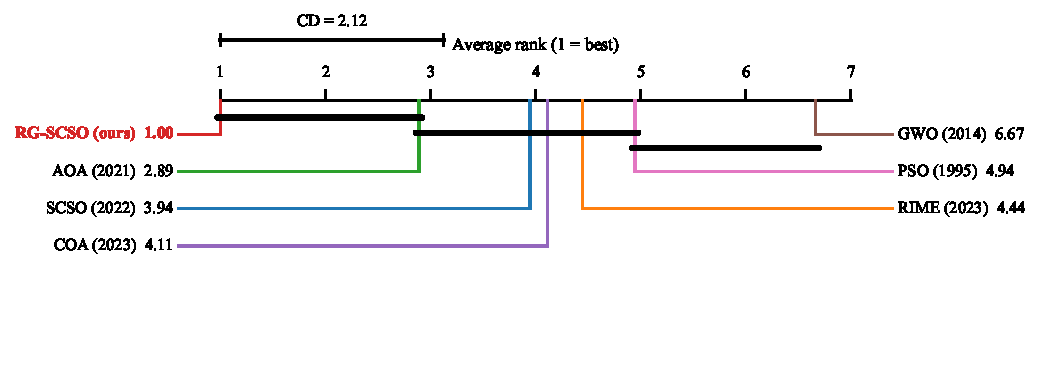
\includegraphics[width=0.92\textwidth]{cd_diagram.pdf}
\caption{Critical-difference (Nemenyi) diagram at $\alpha=0.05$ over the
in-sample ranking (an optimistic upper bound; main text Fig.~2 gives the
held-out counterpart); algorithms not joined by a bar differ significantly in
mean in-sample rank.}
\label{fig:cdinsample}
\end{figure}

\bibliographystyle{plain}
\bibliography{references}

\end{document}
